\documentclass{extbook}[14pt]
\usepackage{multicol, enumerate, enumitem, hyperref, color, soul, setspace, parskip, fancyhdr, amssymb, amsthm, amsmath, bbm, latexsym, units, mathtools}
\everymath{\displaystyle}
\usepackage[headsep=0.5cm,headheight=0cm, left=1 in,right= 1 in,top= 1 in,bottom= 1 in]{geometry}
\usepackage{dashrule}  % Package to use the command below to create lines between items
\newcommand{\litem}[1]{\item #1

\rule{\textwidth}{0.4pt}}
\pagestyle{fancy}
\lhead{}
\chead{Answer Key for Progress Quiz 3 Version B}
\rhead{}
\lfoot{3148-2249}
\cfoot{}
\rfoot{Spring 2021}
\begin{document}
\textbf{This key should allow you to understand why you choose the option you did (beyond just getting a question right or wrong). \href{https://xronos.clas.ufl.edu/mac1105spring2020/courseDescriptionAndMisc/Exams/LearningFromResults}{More instructions on how to use this key can be found here}.}

\textbf{If you have a suggestion to make the keys better, \href{https://forms.gle/CZkbZmPbC9XALEE88}{please fill out the short survey here}.}

\textit{Note: This key is auto-generated and may contain issues and/or errors. The keys are reviewed after each exam to ensure grading is done accurately. If there are issues (like duplicate options), they are noted in the offline gradebook. The keys are a work-in-progress to give students as many resources to improve as possible.}

\rule{\textwidth}{0.4pt}

\begin{enumerate}\litem{
Construct the lowest-degree polynomial given the zeros below. Then, choose the intervals that contain the coefficients of the polynomial in the form $x^3+bx^2+cx+d$.
\[ -4 + 2 i \text{ and } -3 \]

The solution is \( x^{3} +11 x^{2} +44 x + 60 \), which is option A.\begin{enumerate}[label=\Alph*.]
\item \( b \in [11, 13], c \in [42, 45], \text{ and } d \in [52, 62] \)

* $x^{3} +11 x^{2} +44 x + 60$, which is the correct option.
\item \( b \in [-1, 6], c \in [0, 3], \text{ and } d \in [-13, -2] \)

$x^{3} + x^{2} +x -6$, which corresponds to multiplying out $(x -2)(x + 3)$.
\item \( b \in [-11, -7], c \in [42, 45], \text{ and } d \in [-60, -51] \)

$x^{3} -11 x^{2} +44 x -60$, which corresponds to multiplying out $(x-(-4 + 2 i))(x-(-4 - 2 i))(x -3)$.
\item \( b \in [-1, 6], c \in [5, 16], \text{ and } d \in [9, 15] \)

$x^{3} + x^{2} +7 x + 12$, which corresponds to multiplying out $(x + 4)(x + 3)$.
\item \( \text{None of the above.} \)

This corresponds to making an unanticipated error or not understanding how to use nonreal complex numbers to create the lowest-degree polynomial. If you chose this and are not sure what you did wrong, please contact the coordinator for help.
\end{enumerate}

\textbf{General Comment:} Remember that the conjugate of $a+bi$ is $a-bi$. Since these zeros always come in pairs, we need to multiply out $(x-(-4 + 2 i))(x-(-4 - 2 i))(x-(-3))$.
}
\litem{
Construct the lowest-degree polynomial given the zeros below. Then, choose the intervals that contain the coefficients of the polynomial in the form $ax^3+bx^2+cx+d$.
\[ \frac{1}{5}, \frac{-1}{2}, \text{ and } \frac{-5}{2} \]

The solution is \( 20x^{3} +56 x^{2} +13 x -5 \), which is option D.\begin{enumerate}[label=\Alph*.]
\item \( a \in [17, 24], b \in [44, 46], c \in [-22, -11], \text{ and } d \in [-5, 2] \)

$20x^{3} +44 x^{2} -17 x -5$, which corresponds to multiplying out $(5x + 1)(2x -1)(2x + 5)$.
\item \( a \in [17, 24], b \in [48, 59], c \in [5, 16], \text{ and } d \in [-4, 7] \)

$20x^{3} +56 x^{2} +13 x + 5$, which corresponds to multiplying everything correctly except the constant term.
\item \( a \in [17, 24], b \in [63, 71], c \in [35, 38], \text{ and } d \in [-4, 7] \)

$20x^{3} +64 x^{2} +37 x + 5$, which corresponds to multiplying out $(5x + 1)(2x + 1)(2x + 5)$.
\item \( a \in [17, 24], b \in [48, 59], c \in [5, 16], \text{ and } d \in [-5, 2] \)

* $20x^{3} +56 x^{2} +13 x -5$, which is the correct option.
\item \( a \in [17, 24], b \in [-60, -53], c \in [5, 16], \text{ and } d \in [-4, 7] \)

$20x^{3} -56 x^{2} +13 x + 5$, which corresponds to multiplying out $(5x + 1)(2x -1)(2x -5)$.
\end{enumerate}

\textbf{General Comment:} To construct the lowest-degree polynomial, you want to multiply out $(5x -1)(2x + 1)(2x + 5)$
}
\litem{
Which of the following equations \textit{could} be of the graph presented below?

\begin{center}
    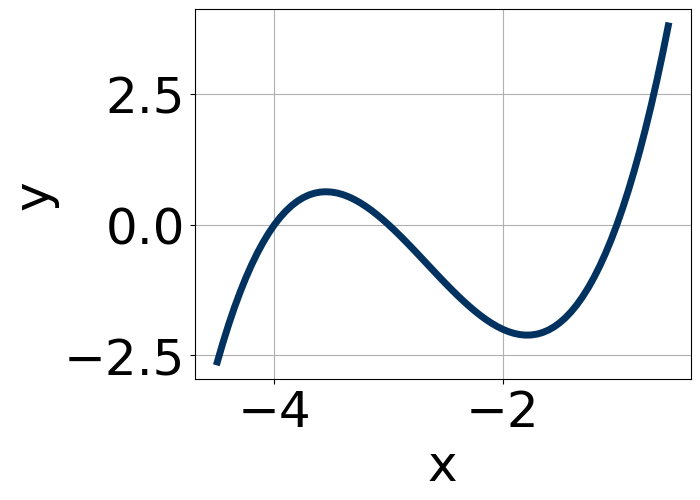
\includegraphics[width=0.5\textwidth]{../Figures/polyGraphToFunctionB.png}
\end{center}




The solution is \( -20x^{7} (x - 3)^{4} (x - 2)^{11} \), which is option D.\begin{enumerate}[label=\Alph*.]
\item \( -4x^{7} (x - 3)^{4} (x - 2)^{6} \)

The factor $(x - 2)$ should have an odd power.
\item \( 14x^{11} (x - 3)^{8} (x - 2)^{11} \)

This corresponds to the leading coefficient being the opposite value than it should be.
\item \( -7x^{5} (x - 3)^{5} (x - 2)^{10} \)

The factor $3$ should have an even power and the factor $2$ should have an odd power.
\item \( -20x^{7} (x - 3)^{4} (x - 2)^{11} \)

* This is the correct option.
\item \( 16x^{8} (x - 3)^{6} (x - 2)^{9} \)

The factor $x$ should have an odd power and the leading coefficient should be the opposite sign.
\end{enumerate}

\textbf{General Comment:} General Comments: Draw the x-axis to determine which zeros are touching (and so have even multiplicity) or cross (and have odd multiplicity).
}
\litem{
Describe the end behavior of the polynomial below.
\[ f(x) = 6(x + 5)^{5}(x - 5)^{8}(x + 9)^{4}(x - 9)^{5} \]

The solution is the graph below, which is option C.
\begin{center}
    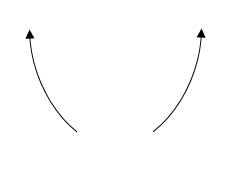
\includegraphics[width=0.3\textwidth]{../Figures/polyEndBehaviorCopyCB.png}
\end{center}\begin{enumerate}[label=\Alph*.]
\begin{multicols}{2}
\item 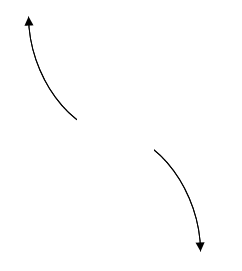
\includegraphics[width = 0.3\textwidth]{../Figures/polyEndBehaviorCopyAB.png}
\item 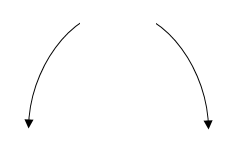
\includegraphics[width = 0.3\textwidth]{../Figures/polyEndBehaviorCopyBB.png}
\item 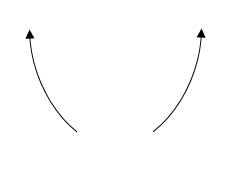
\includegraphics[width = 0.3\textwidth]{../Figures/polyEndBehaviorCopyCB.png}
\item 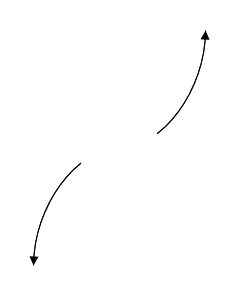
\includegraphics[width = 0.3\textwidth]{../Figures/polyEndBehaviorCopyDB.png}
\end{multicols}\item None of the above.\end{enumerate}
\textbf{General Comment:} Remember that end behavior is determined by the leading coefficient AND whether the \textbf{sum} of the multiplicities is positive or negative.
}
\litem{
Construct the lowest-degree polynomial given the zeros below. Then, choose the intervals that contain the coefficients of the polynomial in the form $ax^3+bx^2+cx+d$.
\[ \frac{-7}{5}, -3, \text{ and } 6 \]

The solution is \( 5x^{3} -8 x^{2} -111 x -126 \), which is option D.\begin{enumerate}[label=\Alph*.]
\item \( a \in [3, 6], b \in [-55, -49], c \in [153, 155], \text{ and } d \in [-130, -115] \)

$5x^{3} -52 x^{2} +153 x -126$, which corresponds to multiplying out $(5x -7)(x -3)(x -6)$.
\item \( a \in [3, 6], b \in [4, 14], c \in [-114, -110], \text{ and } d \in [124, 127] \)

$5x^{3} +8 x^{2} -111 x + 126$, which corresponds to multiplying out $(5x -7)(x -3)(x + 6)$.
\item \( a \in [3, 6], b \in [-11, -4], c \in [-114, -110], \text{ and } d \in [124, 127] \)

$5x^{3} -8 x^{2} -111 x + 126$, which corresponds to multiplying everything correctly except the constant term.
\item \( a \in [3, 6], b \in [-11, -4], c \in [-114, -110], \text{ and } d \in [-130, -115] \)

* $5x^{3} -8 x^{2} -111 x -126$, which is the correct option.
\item \( a \in [3, 6], b \in [-25, -18], c \in [-72, -66], \text{ and } d \in [124, 127] \)

$5x^{3} -22 x^{2} -69 x + 126$, which corresponds to multiplying out $(5x -7)(x + 3)(x -6)$.
\end{enumerate}

\textbf{General Comment:} To construct the lowest-degree polynomial, you want to multiply out $(5x + 7)(x + 3)(x -6)$
}
\litem{
Which of the following equations \textit{could} be of the graph presented below?

\begin{center}
    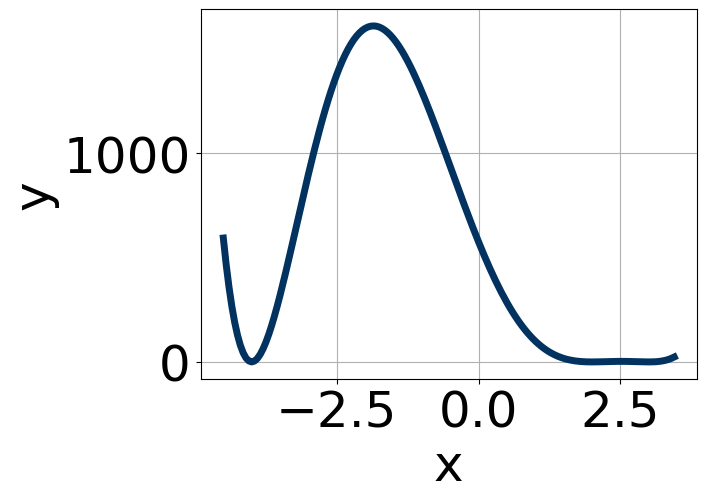
\includegraphics[width=0.5\textwidth]{../Figures/polyGraphToFunctionCopyB.png}
\end{center}




The solution is \( 2(x - 3)^{7} (x + 3)^{9} (x + 4)^{7} \), which is option D.\begin{enumerate}[label=\Alph*.]
\item \( 15(x - 3)^{4} (x + 3)^{10} (x + 4)^{11} \)

The factors $3$ and $-3$ have have been odd power.
\item \( -19(x - 3)^{6} (x + 3)^{9} (x + 4)^{9} \)

The factor $(x - 3)$ should have an odd power and the leading coefficient should be the opposite sign.
\item \( 15(x - 3)^{6} (x + 3)^{9} (x + 4)^{7} \)

The factor $3$ should have been an odd power.
\item \( 2(x - 3)^{7} (x + 3)^{9} (x + 4)^{7} \)

* This is the correct option.
\item \( -10(x - 3)^{7} (x + 3)^{11} (x + 4)^{11} \)

This corresponds to the leading coefficient being the opposite value than it should be.
\end{enumerate}

\textbf{General Comment:} General Comments: Draw the x-axis to determine which zeros are touching (and so have even multiplicity) or cross (and have odd multiplicity).
}
\litem{
Describe the zero behavior of the zero $x = 5$ of the polynomial below.
\[ f(x) = 4(x + 5)^{5}(x - 5)^{8}(x - 2)^{4}(x + 2)^{8} \]

The solution is the graph below, which is option C.
\begin{center}
    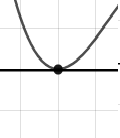
\includegraphics[width=0.3\textwidth]{../Figures/polyZeroBehaviorCB.png}
\end{center}\begin{enumerate}[label=\Alph*.]
\begin{multicols}{2}
\item 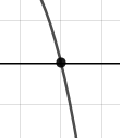
\includegraphics[width = 0.3\textwidth]{../Figures/polyZeroBehaviorAB.png}
\item 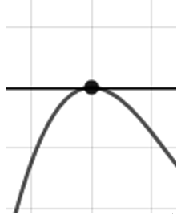
\includegraphics[width = 0.3\textwidth]{../Figures/polyZeroBehaviorBB.png}
\item 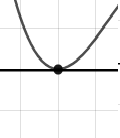
\includegraphics[width = 0.3\textwidth]{../Figures/polyZeroBehaviorCB.png}
\item 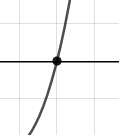
\includegraphics[width = 0.3\textwidth]{../Figures/polyZeroBehaviorDB.png}
\end{multicols}\item None of the above.\end{enumerate}
\textbf{General Comment:} You will need to sketch the entire graph, then zoom in on the zero the question asks about.
}
\litem{
Construct the lowest-degree polynomial given the zeros below. Then, choose the intervals that contain the coefficients of the polynomial in the form $x^3+bx^2+cx+d$.
\[ 5 - 3 i \text{ and } -2 \]

The solution is \( x^{3} -8 x^{2} +14 x + 68 \), which is option C.\begin{enumerate}[label=\Alph*.]
\item \( b \in [0, 5], c \in [-4, 2], \text{ and } d \in [-16, -1] \)

$x^{3} + x^{2} -3 x -10$, which corresponds to multiplying out $(x -5)(x + 2)$.
\item \( b \in [6, 12], c \in [8, 22], \text{ and } d \in [-76, -63] \)

$x^{3} +8 x^{2} +14 x -68$, which corresponds to multiplying out $(x-(5 - 3 i))(x-(5 + 3 i))(x -2)$.
\item \( b \in [-8, -4], c \in [8, 22], \text{ and } d \in [63, 75] \)

* $x^{3} -8 x^{2} +14 x + 68$, which is the correct option.
\item \( b \in [0, 5], c \in [4, 13], \text{ and } d \in [-1, 10] \)

$x^{3} + x^{2} +5 x + 6$, which corresponds to multiplying out $(x + 3)(x + 2)$.
\item \( \text{None of the above.} \)

This corresponds to making an unanticipated error or not understanding how to use nonreal complex numbers to create the lowest-degree polynomial. If you chose this and are not sure what you did wrong, please contact the coordinator for help.
\end{enumerate}

\textbf{General Comment:} Remember that the conjugate of $a+bi$ is $a-bi$. Since these zeros always come in pairs, we need to multiply out $(x-(5 - 3 i))(x-(5 + 3 i))(x-(-2))$.
}
\litem{
Describe the zero behavior of the zero $x = 9$ of the polynomial below.
\[ f(x) = -5(x + 9)^{2}(x - 9)^{3}(x - 8)^{2}(x + 8)^{5} \]

The solution is the graph below, which is option A.
\begin{center}
    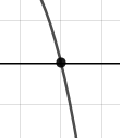
\includegraphics[width=0.3\textwidth]{../Figures/polyZeroBehaviorCopyAB.png}
\end{center}\begin{enumerate}[label=\Alph*.]
\begin{multicols}{2}
\item 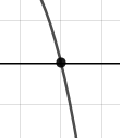
\includegraphics[width = 0.3\textwidth]{../Figures/polyZeroBehaviorCopyAB.png}
\item 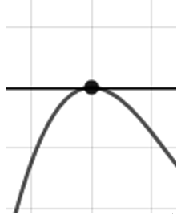
\includegraphics[width = 0.3\textwidth]{../Figures/polyZeroBehaviorCopyBB.png}
\item 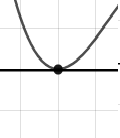
\includegraphics[width = 0.3\textwidth]{../Figures/polyZeroBehaviorCopyCB.png}
\item 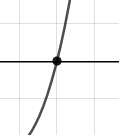
\includegraphics[width = 0.3\textwidth]{../Figures/polyZeroBehaviorCopyDB.png}
\end{multicols}\item None of the above.\end{enumerate}
\textbf{General Comment:} You will need to sketch the entire graph, then zoom in on the zero the question asks about.
}
\litem{
Describe the end behavior of the polynomial below.
\[ f(x) = 8(x + 2)^{5}(x - 2)^{8}(x + 3)^{2}(x - 3)^{2} \]

The solution is the graph below, which is option D.
\begin{center}
    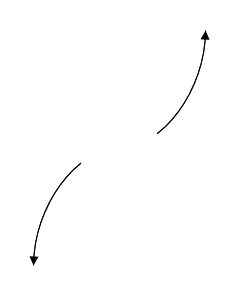
\includegraphics[width=0.3\textwidth]{../Figures/polyEndBehaviorDB.png}
\end{center}\begin{enumerate}[label=\Alph*.]
\begin{multicols}{2}
\item 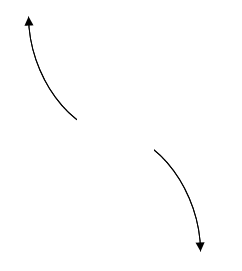
\includegraphics[width = 0.3\textwidth]{../Figures/polyEndBehaviorAB.png}
\item 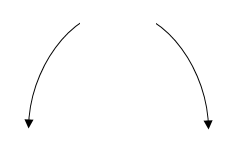
\includegraphics[width = 0.3\textwidth]{../Figures/polyEndBehaviorBB.png}
\item 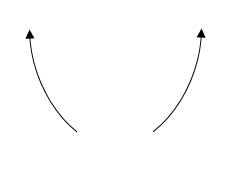
\includegraphics[width = 0.3\textwidth]{../Figures/polyEndBehaviorCB.png}
\item 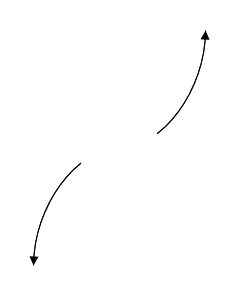
\includegraphics[width = 0.3\textwidth]{../Figures/polyEndBehaviorDB.png}
\end{multicols}\item None of the above.\end{enumerate}
\textbf{General Comment:} Remember that end behavior is determined by the leading coefficient AND whether the \textbf{sum} of the multiplicities is positive or negative.
}
\end{enumerate}

\end{document}